\title{大学入試センター試験数学1・Aを用いた数式処理システムの性能評価}
\author{プロジェクトマネジメントコース\\
ソフトウェア開発管理グループ\\
矢吹研究室\\
1242116\\
森谷慧士}
\date{}
\begin{document}
\maketitle

\chapter*{謝辞}

本研究を進めるにあたり,矢吹研究室矢吹太朗准教授には,多くの時間をご指導にさいて頂きました.また 矢吹研究室の皆様には,多くの知識や示唆を頂きました.協力していただい皆様に感謝の気持ちと御礼を申し 上げます.

\tableofcontents%目次

\chapter{序論}


東京大学の入試問題を全自動で解くプロジェクト(東ロボプロジェクト)が進められている\cite{arai2014}.

\begin{figure}[h]
\centering
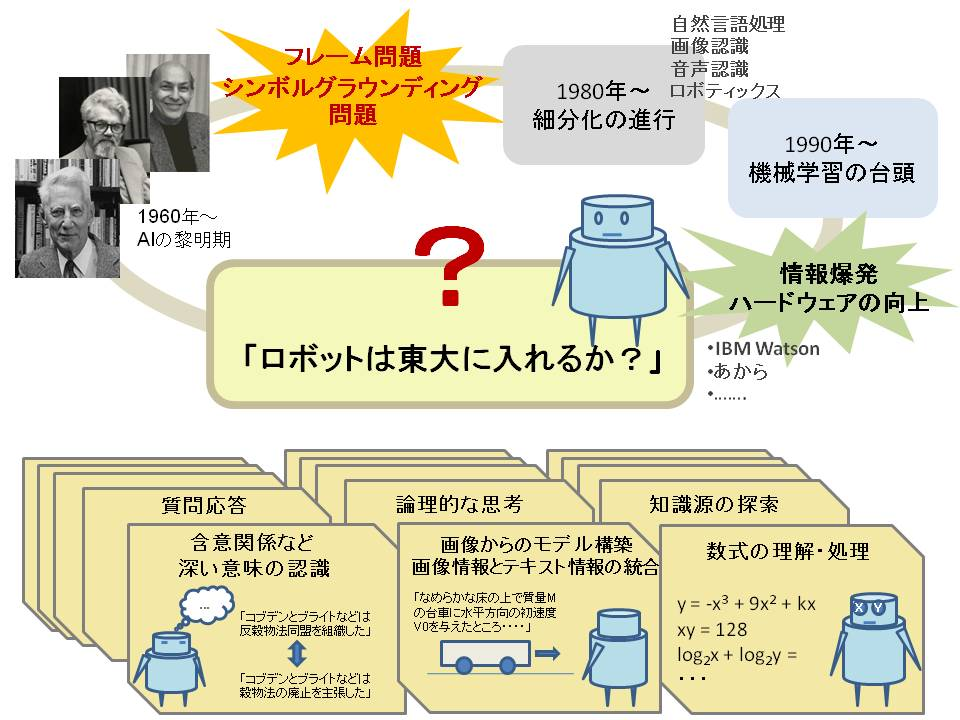
\includegraphics[width=15cm]{tourobo.jpg}
\caption{東ロボプロジェクト}\label{図}
\end{figure}

このプロジェクトは,国立情報学研究所(大学共同利用機関法人 情報・システム研究機構)が,中心となって1980年以降細分化された人工知能分野を再統合することで新たな地平を切り拓くことを目的に,若い人たちに夢を与えるプロジェクトとして発足した\cite{tourobo}.

このプロジェクトの具体的なベンチマークとして,2016年度までに大学入試センター試験で高得点をマークすること,また2021年度に東京大学入試を突破することを目標に研究活動を進めている.

これまで蓄積された人工知能の各要素技術の精度を高め,情報技術分野の未来価値創成につなげるとともに,人間の思考に関する包括的な理解を内外の研究者とともに深めることを目標としている.また,本プロジェクトでは,日本における学際的な知識・先端技術を集積するだけでなく,国際的な連携も視野に入れ,研究活動を進めている.

\clearpage

ここでは,東ロボプロジェクトの中でも特に数学について紹介する.

東ロボは,情報処理技術の観点から人間の知能に対するアプローチの一つとして取り組んでおり,数学入試問題で東大入試に合格できるレベルの技術を作ることを目的としている.



東ロボでは,NIIと富士通研究所が共同で,問題文を認識・解釈しコンピュータが理解できるデータの形にする数式認識や,数式処理ソルバが理解できる式表現を立式するための自然言語処理,立式された問題を高速に正確に解くための数式処理技術など,人間中心のITを実現するために必要な技術の開発を行い,目標達成を目指している.このプロジェクトで開発された技術により,高度な数理解析技術が誰にでも容易に使えるようなものになることが期待される.

東ロボプロジェクトでは,数学の問題を解く過程を以下の3つの手順にしている.

\begin{enumerate}
\item 人間にとって理解しやすい自然言語や数式で表現された問題文を理解する.

\item コンピュータが処理できる形式に変換する.

\item 数式処理ソルバで答えを求める.
\end{enumerate}

この手順を図で示すと図1のようになる.

\begin{figure}[h]
\centering
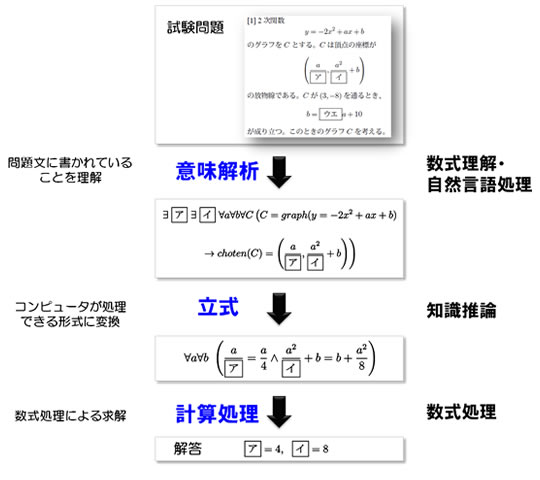
\includegraphics[width=15cm]{10b.jpg}
\caption{数学を解くための手順}\label{図}
\end{figure}

人間が理解するようにコンピュータが言葉を理解することは容易ではない.自然言語処理によって導かれる問題文の意味表現を,コンピュータが処理できる形式で立式を行うには,問題文の言語解析だけではなく,数学の用語や高校数学知識をうまく統合することが必須である.また,与えられた問題に対してコンピュータがどう解けばよいのか自ら判断することも求められる.立式ができた後にコンピュータで求解する部分については,大学入試2次試験の数学の問題について数式処理技術を使ってもおおよそ5~6割しか解けないのが現状であり,計算アルゴリズムの高度化も重要である.

このように,各ステップにおいてさまざまな理論・技術の開発が必要であり,それらの技術を問題ごとに適切に組み合わせ繋いでいくことも必要になる.

\clearpage

次に,東ロボプロジェクトが2015年度のセンター試験に挑戦した際の結果を記述する.

東ロボは,センター試験の模擬試験で,5教科8科目で511点を記録し,偏差値57.8を獲得した.特に,数学と世界史では偏差値60を超え,数学Ⅰ・A は偏差値64,数学Ⅱ・Bは偏差値65.8,世界史は偏差値66.5を記録した.

さらに,東大入試試験の模擬試験では,世界史に挑戦し偏差値54.1を記録した\cite{tourobo}.

\begin{figure}[h]
\centering
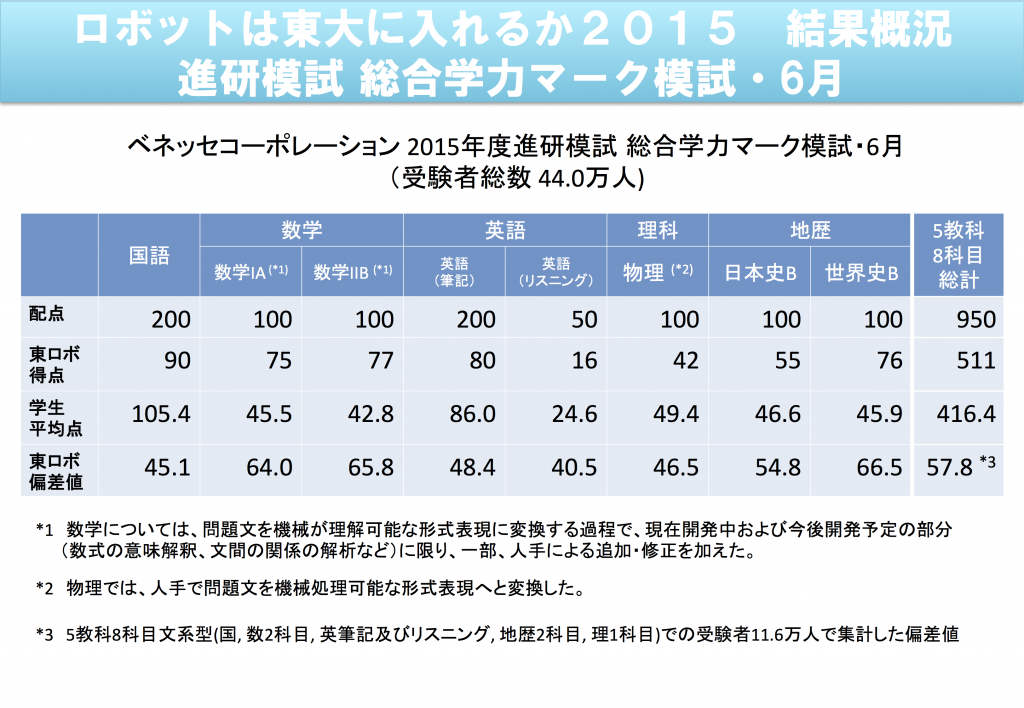
\includegraphics[width=15cm]{TOROBO2015gaikyo_1.png}
\caption{東ロボのセンター試験形式模試の結果}\label{図}
\end{figure}


\begin{figure}[h]
\centering
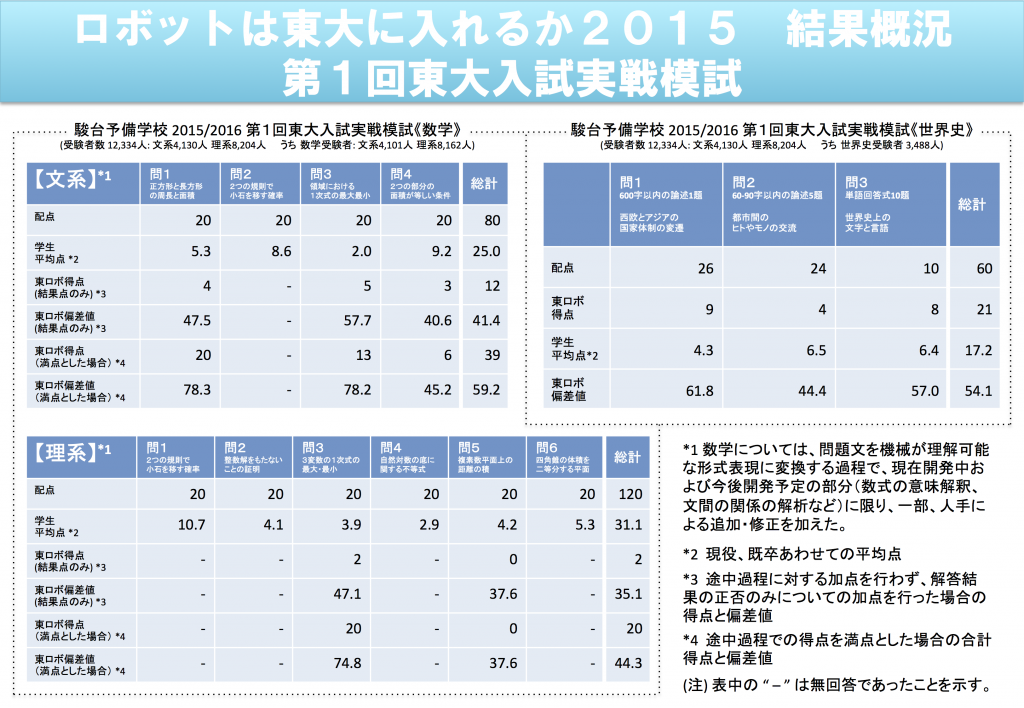
\includegraphics[width=15cm]{TOROBO2015gaikyo_2.png}
\caption{東ロボの二次試験形式模試の結果}\label{図}
\end{figure}




人工知能がこのように発達すると,その影響は数学教育にも及ぶだろう.
今日の数学教育は,すべてを紙と鉛筆で行うことを前提に行われているが,その一部は コンピュータで置き換えることができるはずである.
人間が行うこととコンピュータが行うことをうまく識別する能力の育成が求められるようになるだろう.



\chapter{背景}

\section{第4の産業革命}
政府が進めているプロジェクトがある.「第4の産業革命」というロボットや,人工知能を活用した革新的なものづくりを目指す取り組みが始まった\cite{sangyou2014}.
この取り組みは,ドイツで「インダストリー4.0」と呼ばれる動きから始まり,日本政府も経済産業省を中心に取り組まれ始めている.

\begin{figure}[h]
\centering
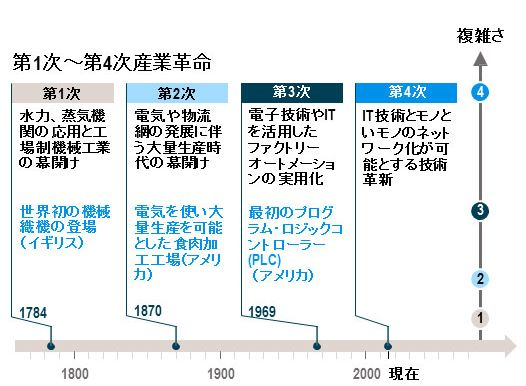
\includegraphics[width=15cm]{sanngyou.jpg}
\caption{第4の産業革命}\label{図}
\end{figure}

インダストリー4.0とは,インターネットと人工知能の本格的な導入によって,生産・供給システムの自動化,効率化を革命的に高めようとし,生産工程のデジタル化・自動化・バーチャル化のレベルを現在よりも大幅に高めることで,コストの極小化を目指すというものである.現在ドイツの電子機器メーカーや自動車メーカー,IT・通信企業が必死に取り組んでいるのが,スマート工場つまり「自ら考える工場」の開発である\cite{nikkeionline}.

\begin{figure}[h]
\centering
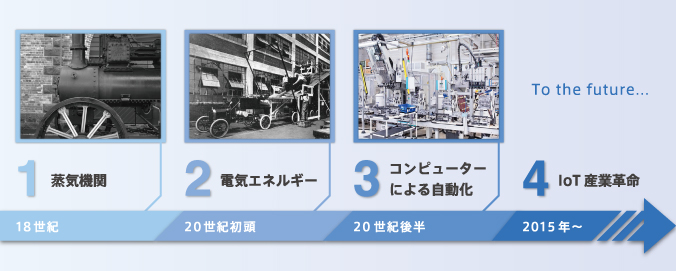
\includegraphics[width=15cm]{005.jpg}
\caption{第4の産業革命2}\label{図}
\end{figure}

\clearpage

\section{ソフトバンクのPepper}

2015年2月には,ソフトバンクが人工知能を搭載したヒト型ロボットの「Pepper」を発売した.Pepperは,感情認識と自立感情を持つロボットである.本体に搭載された各種センサーで状況を判断し,独自のアルゴリズムでロボットの機能を制御するアプリを自律的に制御する.




また,カメラや音声認識技術によって人の表情と声からその人の感情を推定する感情認識機能も搭載している.これにより,Pepperは人とコミュニケーションを通じて和ませ,喜ばすことが可能となる.今後は,ネットワークと接続し,更に進化することが望まれる\cite{softbank}.

\begin{figure}[h]
\centering
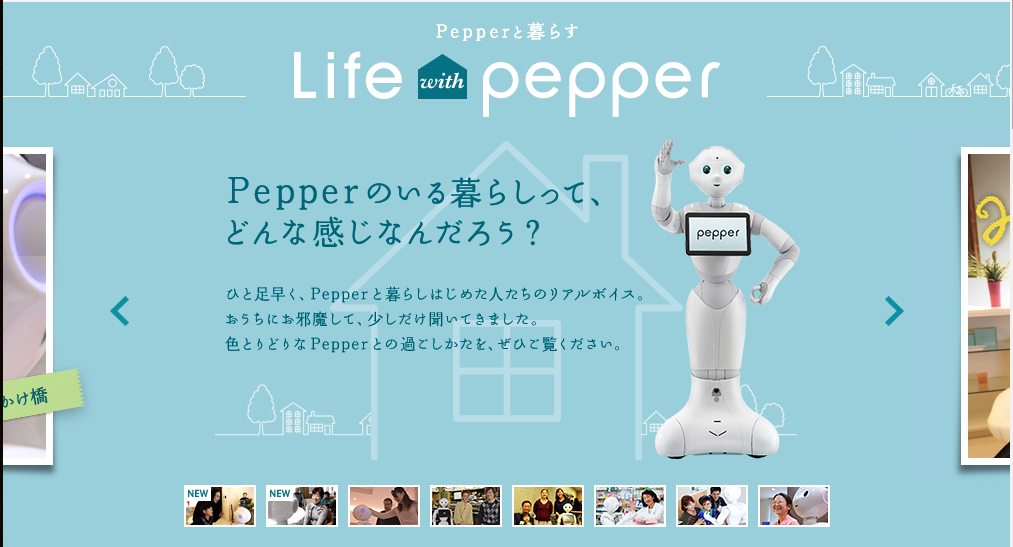
\includegraphics[width=15cm]{pepper.png}
\caption{ソフトバンクのPepper}\label{図}
\end{figure}

Pepperとは,感情認識ヒューマノイドロボットである.フランスのアルデバランロボティクスと同社に出資するソフトバンクグループ傘下のソフトバンクモバイルにより共同開発された.Pepperは,感情エンジンとクラウドAIを搭載した世界初の感情認識パーソナルロボットである.OSはNAOqiというOSを採用し、Naoにはプラットフォームの互換性がある.

\begin{figure}[h]
\centering
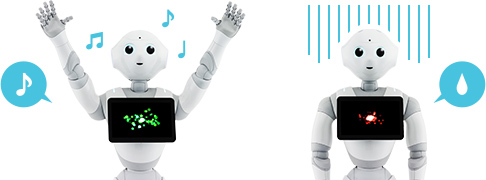
\includegraphics[width=15cm]{figemotion2.jpg}
\caption{pepperの感情表現}\label{図}
\end{figure}

\begin{figure}[h]
\centering
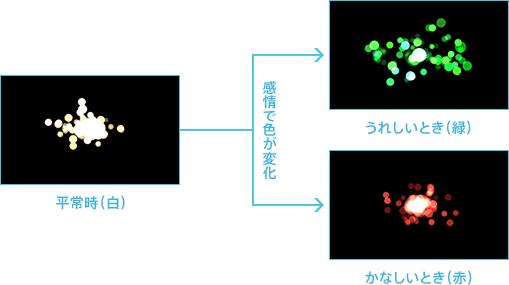
\includegraphics[width=15cm]{figemotion3.png}
\caption{pepperの感情表現}\label{図}
\end{figure}

\begin{figure}[h]
\centering
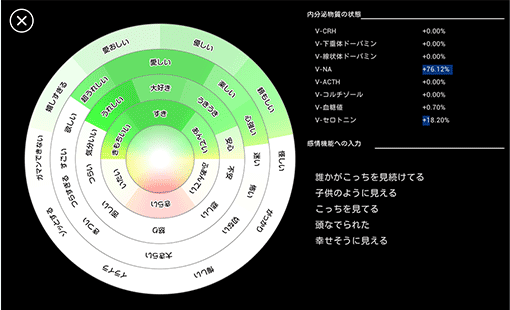
\includegraphics[width=15cm]{figemotion4.png}
\caption{pepperの感情表現の詳細}\label{図}
\end{figure}


Pepperには表情と声からその人の感情を察する「感情認識機能」が備わっているだけでなく、独自の感情機能により,自ら感情を持ち行動する,そして将来的には人とロボットの心が通い合う存在になることを目指したロボットである.

\begin{figure}[h]
\centering
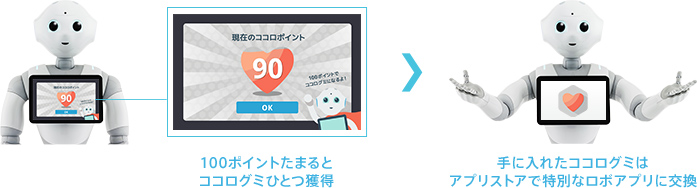
\includegraphics[width=15cm]{figemotion6.jpg}
\caption{ココロミグ}\label{図}
\end{figure}

Pepperは,新しいロボアプリをアプリストアから自由にダウンロードして,できることのバリエーションを増やしていける.また,Pepperとふれあったり,一緒に遊んだりすると得られる「ココログミ」を使うことで,アプリストアで特別なロボアプリを手に入れることもできる.さらに,開発環境も公開されているので,自分ならではのロボアプリを作って楽しむことも可能であり,今後もさまざまなロボアプリがアプリストアに追加され,人工知能の開発において大きな期待が見込まれる.

\clearpage


\section{コールセンターにWatsonを導入}

2014年11月にはみずほ銀行がコールセンターにIBMの人工知能であるWatsonを導入したことが話題となった.みずほ銀行では、人工知能を利用することで,膨大な解答例データの中から最適な回答案を優先的に表示させ,コールセンターの対応時間の短縮につなげることができる.このように,ビジネス内での様々なシステムに人工知能が導入され始めている\cite{mizuho2014}.

\begin{figure}[h]
\centering
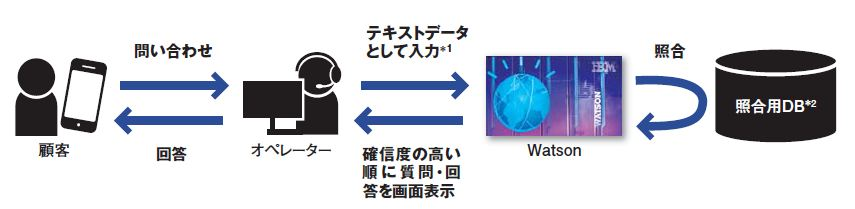
\includegraphics[width=15cm]{watson.jpg}
\caption{コールセンター業務でのWatson活用の流れ}\label{図}
\end{figure}


ここで,コールセンターに利用されたWatsonについて紹介する\cite{watson}.

Watsonは,IBMが開発した質問応答システム,意思決定支援システムである.IBM自体はWatsonのことを,自然言語を理解・学習し人間の意思決定を支援する「Cognitive Computing System」と定義しており,一般的な人工知能とは少し違うものであるとしている.Watsonが初めて公に出たのが,アメリカのクイズ番組に出演した時である.クイズ番組では,自然言語を文脈を含めて質問の趣旨を理解し,人工知能として大量の情報の中から適切な回答を選択し,回答する方法がとられた.将来的には,医療などの分野での活躍が期待される.




\chapter{目的}

本研究では,大学入試センター試験数学I・Aを題材にして,数学教育にコンピュータを導入することの可能性を調査する.

その結果として,高校程度の数学能力を問う問題でコンピュータを活用して解く際に必要となる数学の知識とコンピュータの知識を明らかにすることを目指す.

\chapter{プロジェクトマネジメントとの関連}

プロジェクトを進める際に,プロジェクトメンバの一人として人工知能を導入する.また,ステークホルダーとして人工知能を導入する.これらの動作をすることで,プロジェクトマネージャを人工知能が補佐することが出来る.

\chapter{手法}

本研究では,センター試験の数学I・A の問題をコンピュータを用いて解き,問題を解くために必要な数学の知識とコンピュータの知識を確認する.



\section{コンピュータシステム}

解答にはコンピュータシステムは数式処理システムMathematicaを用いる.

コンピュータを数学に応用する方法は,低水準言語から高水準言語まで,さまざまなレベルが考えられるが,本研究では,人間が書く答案と抽象度が最も近いと思われる数式処理システムを検討し,数式処理システムの中で最も普及しているものの一つであるMathematicaを採用する.

Wolfram言語の実行環境をMathematicaと呼ぶこともあるが,本稿では言語自体もMathematicaと呼ぶ.

Mathematicaには,Windows版とMac版,Linux版,Raspberry Pi版,クラウドサービス版があるが,本研究では,無料で利用できるクラウドサービス版,Wolfram ProgrammingLab\footnote{\url{https://lab.open.wolframcloud.com/objects/wpl/GetStarted.nb}}を用いる.

\clearpage

\section{解答方法}

ここでは,本研究で数学の問題を解く過程を解説する.

数式処理システムを用いて数学の問題を解く例として,「$x$についての方程式$f(x)=x^2-ax+5=0$が重解を持つような$a$の値を求めよ」という問題を,2通りの方法で解く.

第1の方法は,方程式が重解を持つことと判別式$a^2-20$が$0$であることが同値だと考え,$a$についての方程式$a^2-20=0$を解くというものである.方程式を解くためには,Mathematicaの\verb|Solve[|方程式\verb|, |変数\verb|]|という記法を用いる.\cite{wolfram2014}.

\begin{verbatim}
Solve[a^2 - 20 == 0, a]
\end{verbatim}

\vspace{-5mm}\[\left\{\left\{a\to -2 \sqrt{5}\right\},\left\{a\to 2 \sqrt{5}\right\}\right\}\]

この結果は,$a$が$-2\sqrt{5}$または$2\sqrt{5}$であることを表している.

第2の方法は,2次方程式が重解を持つということをMathematicaが処理可能な形式に変換し,その記述を評価するというものである.

2次方程式が重解を持つというのは,「ある解$x_1$が存在し,すべての解$x_2$は$x_1$と等しい」と言い換えられる.
この命題を論理式で書くと$\exists x_1\;f(x_1)=0\land\left(\forall x_2\;f(x_2)=0\to x_2=x_1\right)$となる.\verb|Exists|や\verb|ForAll|を使ってこの命題を記述し,そこから限定子を除去すると$a$の値が求まる.限定子の除去には\verb|Reduce|を用いる.

\begin{verbatim}
Reduce[
 Exists[x1, f[x1] == 0,
  ForAll[x2, f[x2] == 0, x2 == x1]],
 a]
\end{verbatim}

\vspace{-5mm}\[a=-2 \sqrt{5}\lor a=2 \sqrt{5}\]

この結果も,$a$が$-2\sqrt{5}$または$2\sqrt{5}$であることを表している.

センター試験の問題は,紙と鉛筆で解けるように作られているため,そこにコンピュータを持ち込んでももちろん解ける.

本研究では,問題をなるべく素直に解釈して解くことにする.

上述の例では,判別式を思いつかなければならない第1の解法よりも,問題の表現を機械的に翻訳すればよい第2の解法を採用する.

\clearpage

\section{研究過程}

本研究では,大学入試センター試験の数学にMathematicaを用いて解く.そして,使用したシンボルの数と,利用した数学的知識を集計する.

その際に,数学の問題を解く過程を二つにする.


\begin{enumerate}
\item 数学の問題を理解し,数学的知識を利用して計算式などの数学的表現に変換する過程である.

\item 数学的表現に変換した式を数式処理して,値を求める過程である.
\end{enumerate}

今回は後者を人工知能に処理させ,前者を人間が処理するように分ける.その際に,人間がいかに簡潔に問題文を処理できるかを研究する.

第一工程では,大学入試センター試験の数学の問題をできるだけ人間が頭を使わずに,素直に数学的表現に翻訳する.

第二工程では,第一工程で数学的表現に翻訳した式をMathematica に与えて数式処理を行う.この工程では,Mathematica が式を最適に処理できるコードを与えて,最適解を得る.この際に,使用したコードの種類を集計し,統計を取る.

大学入試センター試験の問題は,紙と鉛筆だけで解けるように作られているため,そこにコンピュータを導入してももちろん解ける.そこで本研究では,問題をそのまま素直に解釈して,Mathematicaで解くようにする.

例えば,「二次関数$3a^2 -6a-36==-27$を解け」という問題を解く.この問題には,Solveというコードを用いる.このSolveは,方程式の解を求めるのに用いられる.\[Solve[3a^2 -6a-36==-27,a]\]とMathematicaに打ち込み,解かせると,\[{{a→-1},{a→3}}\]という答えが帰ってくる.

次に,「二次不等式$2a^2 -6a-36<=0$を解け」という問題を解く.この問題には,Reduceというコードを用いる.このReduceは,方程式あるいは不等式を解き,限定子を除去することで命題を簡約する.\[Reduce[2a^2 -6a-36<=0,a]\]とMathematicaに打ち込むと,\[-3<=a<=6\]という答えが帰ってくる.

例のように,問題に対して的確なコードを探しだし,Mathematicaを用いて解くという方法を用いる.

\clearpage

\section{問題処理の例}

ここでは,例として大学入試センター試験から以下の問題を処理する.
例題

以下では,a=756とする.

Aを素因数分解すると
$A=2^ア・3^イ・ウ$
である.

Aの正の約数の個数はエオ個である.

この問題を処理する.

この問題では,第一工程として,Mathematicaに打ち込む値を設定する.

次に,第二工程として今回利用するシンボルを設定する.

ここでは,FactorIntegerとDivisorsとLengthのシンボルを利用する.

まずは,問題を素因数分解し空欄の「ア・イ・ウ」に答えを埋める.

\[a=756\]

これで,問題と同じ756という整数を$a$と置く.

\[FactorInteger[a]\]
\[{{2,2},{3,3},{7,1}}\]
と処理される.この${2,2}$は$2^2$ということなので,ア=2,イ=3,ウ=7となる.

次に,正の約数の個数「エオ」を求める.

\[b=Divisors[a]\]
\[{1,2,3,4,6,7,9,12,14,18,21,27,28,36,42,54,63,84,108,126,189,252,378,756}\]

これで,756の約数すべてが表示される.表示されたリストを「b」として次に

\[Length[b]\]
\[24\]

を打ち込むことで,24と表示される.

出力された解を,紙で解いた回答と合わせ正解ならば,ここでこの問題の処理は終了する.このように,問題ごとに各工程の作業を行い調査する.

\clearpage

\section{集計}

問題を解いたら,その際に用いたMathematicaの組み込みシンボルの種類を数える.

たとえば,上述の第2の解法では,\verb|Reduce|と\verb|Exists|,\verb|ForAll|という3種の組み込みシンボルを用いている(厳密に言えば,\verb|x2 == x1|は正式には\verb|Equal[x2, x1]|と記述されるため,\verb|Equal|も数えるべきではあるが,ここでは「\verb|==|」のような自明なものは数えないことにする).

初めのうちは,問題の数が増えるにつれて,利用する組み込みシンボルの種類も増えるが,センター試験の数学I・Aの問題を解くのに使える組み込みシンボルが出尽くせば,シンボルの種類の増加は止まるはずである.


\chapter{大学入試センター試験}

\section{大学入試センター試験とは}
大学入試センター試験とは,独立行政法人大学入試センターが2日間にわたって実施する日本の大学の共通入試試験のことである.

このことより本研究では,大学入試センター試験が日本の多くの大学で採用していることから,知名度が高いことを利用する.ほとんどの受験生が受験する大学入試センター試験を調査の対象とすることで,大学生にもわかりやすくする.

\begin{figure}[h]
\centering
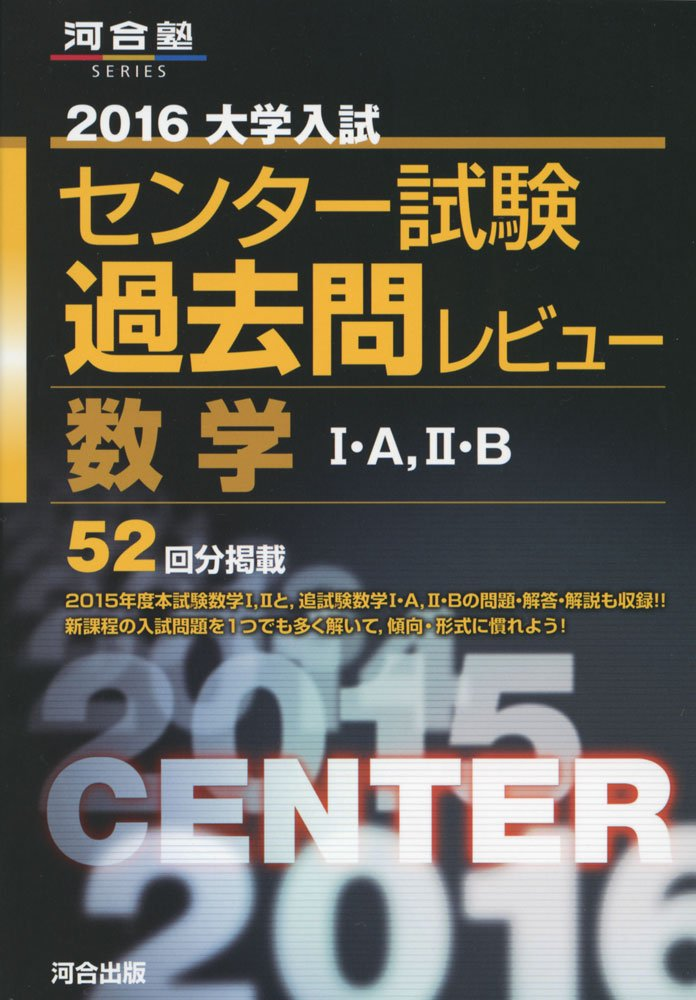
\includegraphics[width=13cm]{center.jpg}
\caption{河合塾 2016 大学入試 センター試験過去問レビュー 数学Ⅰ・A,Ⅱ・B}\label{写真}
\end{figure}

本研究では,河合出版が発刊している「河合塾 2016 大学入試 センター試験過去問レビュー 数学Ⅰ・A,Ⅱ・B」を使用する.本書は,1997年~2015年までの14年分の問題を収録しているため,研究に最適であると考えた.

その中でも本研究では,センター試験の数学I・Aの問題を解くことにする.これは,数学Ⅰ・Aは解きやすく,研究に適していると考えたからである.




\chapter{数式処理システム}

\section{Mathematicaとは}

Mathematicaとは,あらゆる分野の計算に対応する豊富な関数と高度なグラフィック機能を備えた数式所為システムである.Mathematicaを提供しているウルフラム・リサーチ社を創業したスティーブン・ウルフラム氏が考案し広く使われている数式処理システムである.

\begin{figure}[h]
\centering
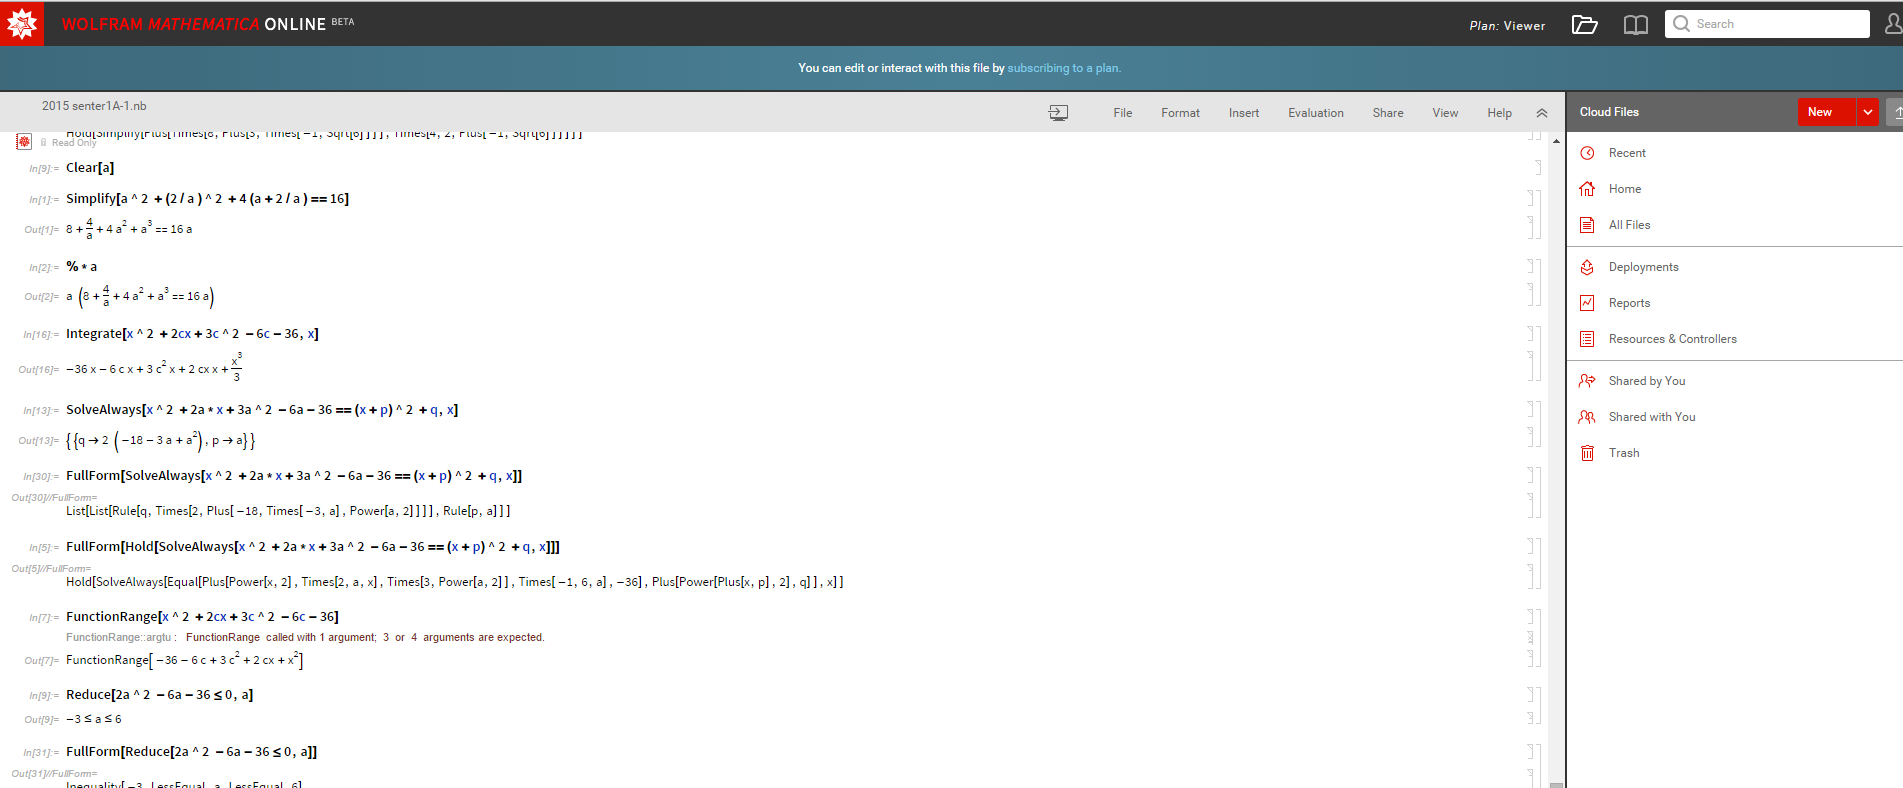
\includegraphics[width=15cm]{mathmatica.png}
\caption{Mathematica 例}\label{図}
\end{figure}

\clearpage

\section{Wolfram言語とは}

Wolfram言語とは,ウルフラム・リサーチ社が開発した,非常に汎用性の高いマルチパラダイムプログラミング言語である.

Mathematicaは,Wolfram言語を利用する.Wolfram言語は,Mathematica独自のノートブックインターフェイス上で利用することで,インタラクティブなデータ処理を行うスクリプトとして利用できる.さらに,アプリケーションの開発言語として利用すれば,GUIから高度な計算エンジンまで,一貫して一つの環境下で開発を行うことが出来る.

Wolfram言語は,汎用的なデータベースやインターネット上のデータを直接取り組むことができ,5000もの組み込み関数を内蔵しているため,わずか数行でも高度なアプリケーションも開発できる.また,Wolfram言語はMathematicaだけでなくWolfram社が無償で提供しているWolfram Alphaでも利用できる.

\begin{figure}[h]
\centering
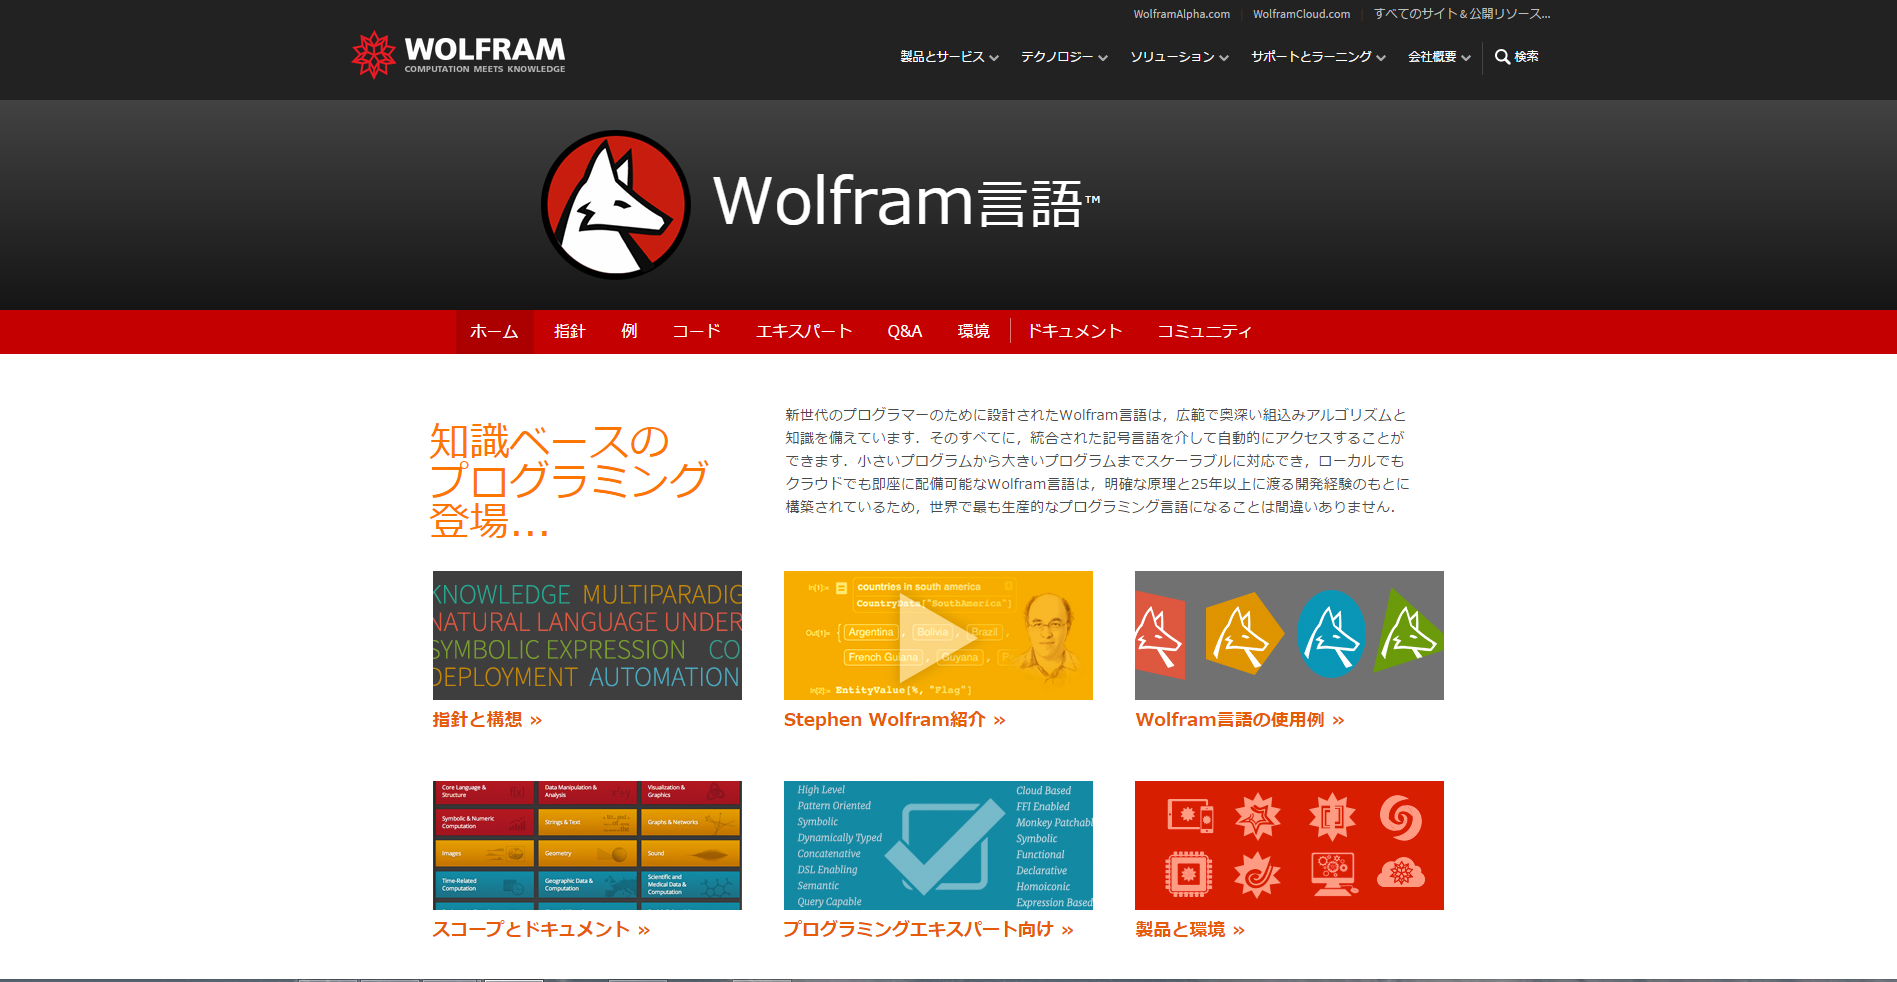
\includegraphics[width=15cm]{wolfram.png}
\caption{Wolfram ホームページ}\label{図}
\end{figure}

\clearpage

\section{Wolfram言語の使用例}

Wolfram言語は,本研究で利用する数式の処理だけでなく,プログラミング言語としても利用されている.

新生代のプログラマーのために設計されたWolfram言語は,広範で奥深いアルゴリズムと知識を備えている.言語のすべてが,統合された記号言語を介して自動的にアクセスすることができる.Wolfram言語は,小さいプログラムから大きいプログラムまで広く対応でき,ローカルでもクラウド上でもすぐに利用可能である.

Wolfram言語は,「Hello World」を表示するような基本的なプログラミングや,手書きの数字の識別,グラフの作成,画像認識,写真から顔の検出,地図の色分け,ある国の人口など様々なことがたった数行のコードで利用可能である.

ここで,「Hello World」を表示する例を紹介する.

\[CloudDeploy["Hello, World"]\]

コードが処理され,URLが表示される.これをクリックすることで「Hello world」が表示される.

\begin{figure}[h]
\centering
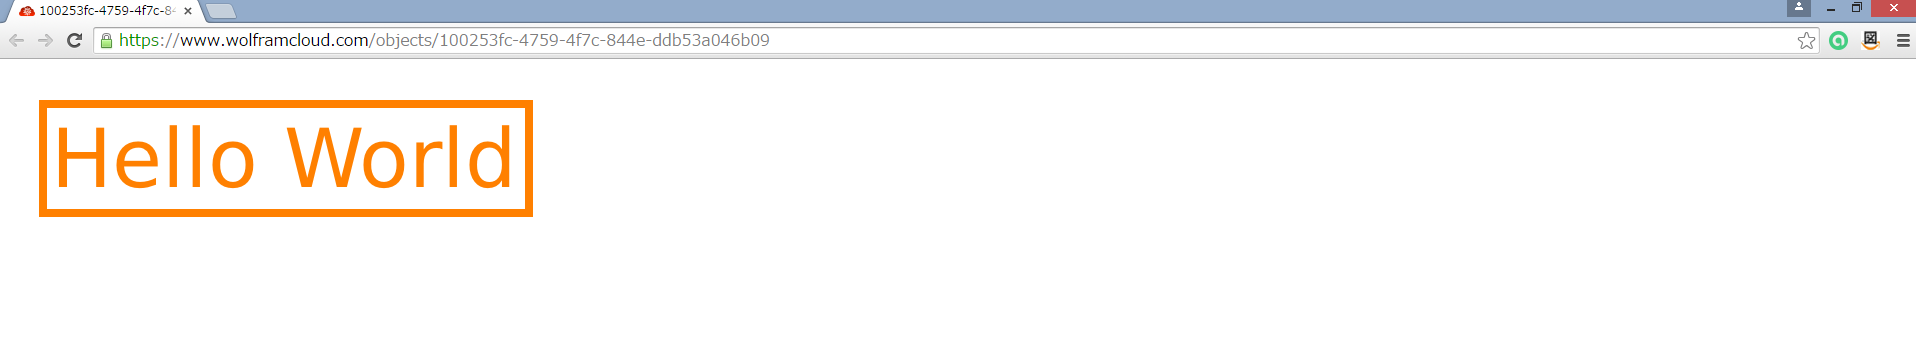
\includegraphics[width=15cm]{helloworld.png}
\caption{Hello World 例}\label{図}
\end{figure}

さらにWolfram言語は,現実のデータを使った計算が可能である.単位や,地理情報,日付,画像,その他何千もの分野で直接計算が可能となる.

このように,Wolfram言語は汎用性が高く少ないシンボルで利用ができるので,世界中で利用され教育の場でも利用されている.

\clearpage

\section{Mathematicaの使用例}

本研究では,Wolfram社が提供するMathematica Onlineを利用する.ここではMathematicaを実際に動かす例を見せる.

まずは環境設定をする.

\begin{figure}[h]
\centering
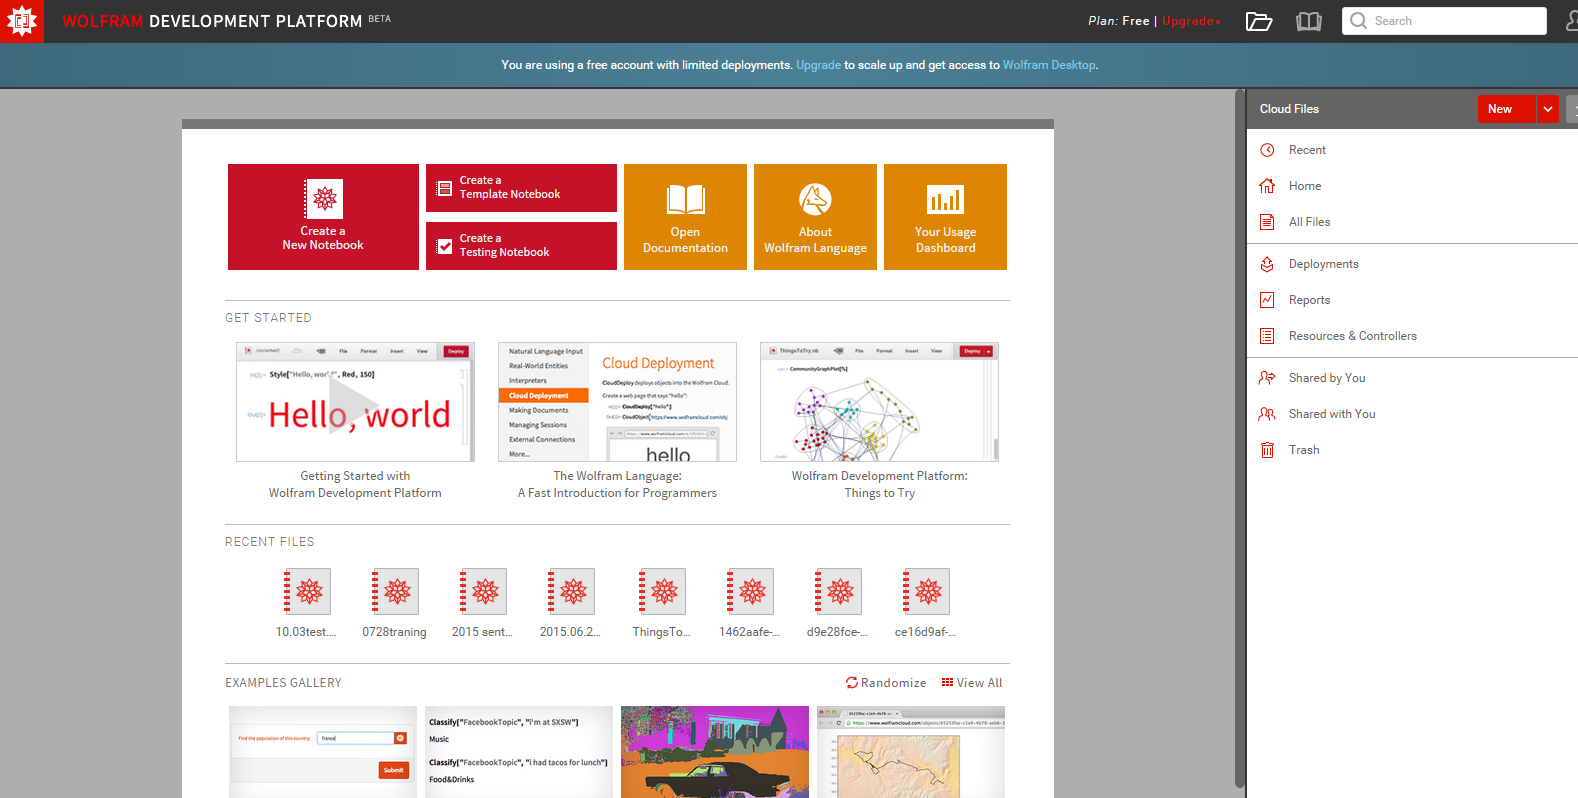
\includegraphics[width=15cm]{mathematica2.png}
\caption{Mathematica 例1}\label{図}
\end{figure}

Wolframのアカウントを作成し,「Create a New Notebook」を押して新しいノートを作成する.

\begin{figure}[h]
\centering
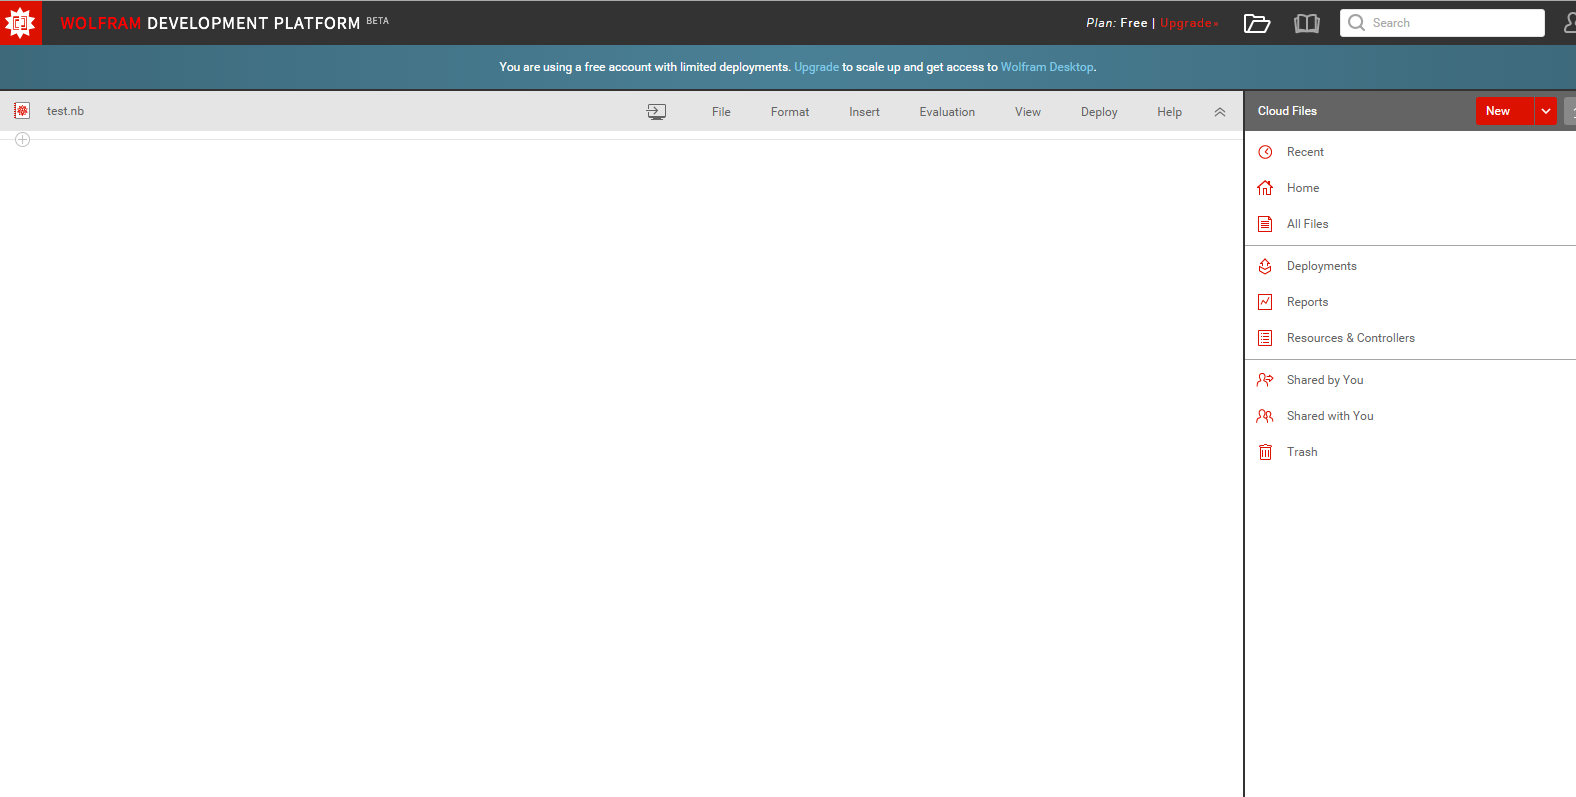
\includegraphics[width=15cm]{mathematica3.png}
\caption{Mathematica 例2}\label{図}
\end{figure}

これが、Mathematica Onlineのノートである.ここに,シンボルと数式を書き込むと,処理をする.

\clearpage

\begin{figure}[h]
\centering
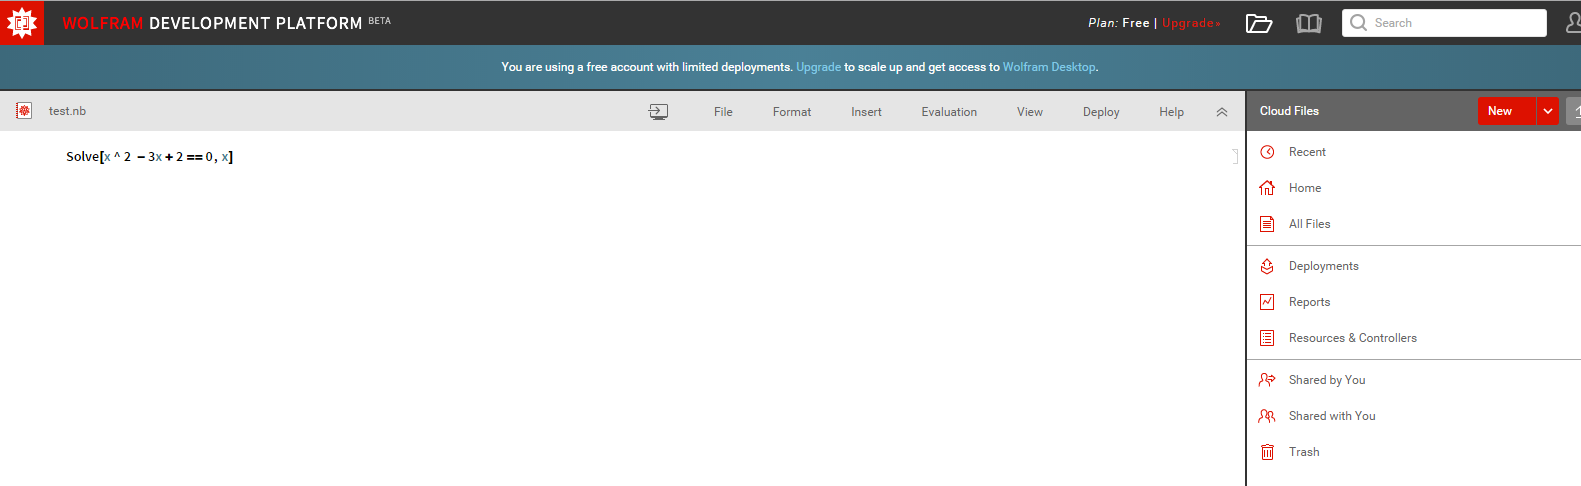
\includegraphics[width=15cm]{mathematica4.png}
\caption{Mathematica 例3}\label{図}
\end{figure}

このように、シンボルと数式を打ちこむ.ここでは,$x^2-3x+2=0$を処理させ,解を求める.

\begin{figure}[h]
\centering
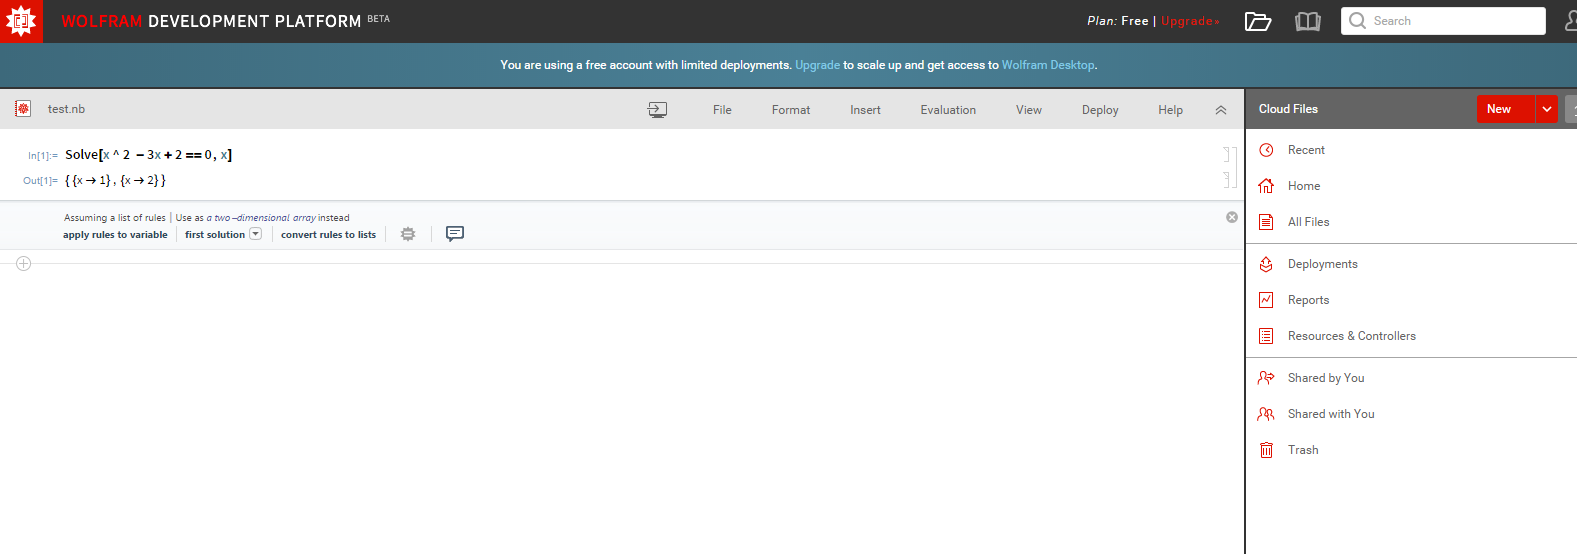
\includegraphics[width=15cm]{mathematica5.png}
\caption{Mathematica 例4}\label{図}
\end{figure}

このように,処理した値が表示される.本研究では,以上のようにMathematicaを利用し,研究を進めていく.


\chapter{調査}

\section{調査方法}

ここでは,調査方法を具体的に説明する.本研究では、前述のとおり数学の問題を解く過程を二つにする.

\begin{figure}[h]
\centering
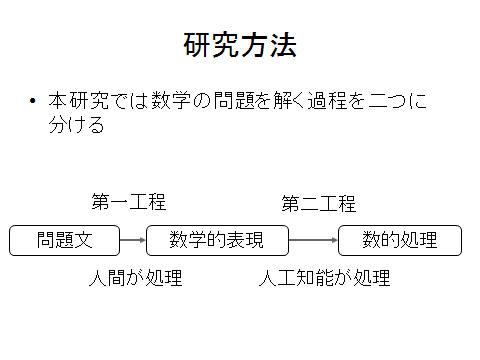
\includegraphics[width=15cm]{katei.png}
\caption{調査過程}\label{図}
\end{figure}

\section{第一工程}

第一工程では,大学入試センター試験の数学の問題をできるだけ人間が頭を使わずに,素直に数学的表現に翻訳する.大学入試センター試験の問題は,受験生が紙と鉛筆だけで解けるように作られているため,出来る限りMathematicaが問題を処理できるように式に変換する.この際に,使用した数学的知識を集計し,統計を取る.

\begin{figure}[h]
\centering
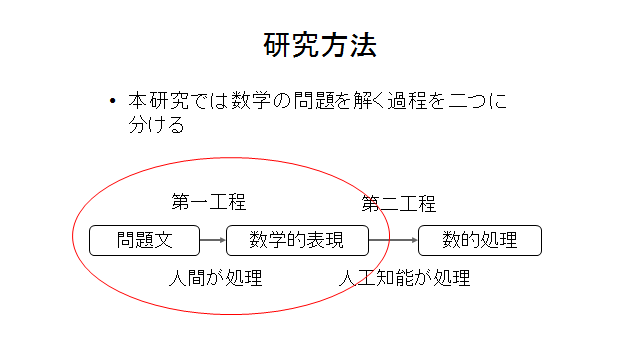
\includegraphics[width=15cm]{katei2.png}
\caption{調査過程}\label{図}
\end{figure}

\section{第二工程}

第二工程では,第一工程で数学的表現に翻訳した式をMathematicaに与えて数式処理を行う.この工程では,Mathematicaが式を最適に処理できるコードを与えて,最適解を得る.この際に,使用したコードの種類を集計し,統計を取る.

\begin{figure}[h]
\centering
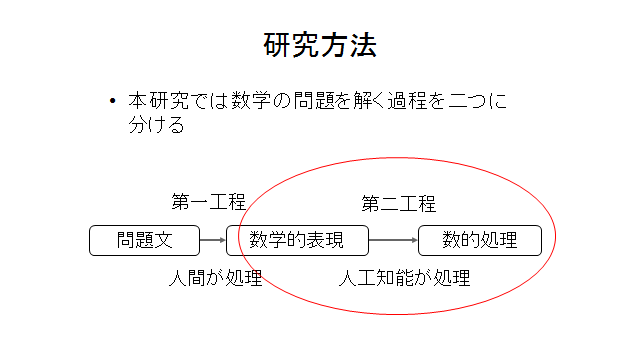
\includegraphics[width=15cm]{katei3.png}
\caption{調査過程}\label{図}
\end{figure}


\chapter{結果}

\begin{figure}[tb]
\centering
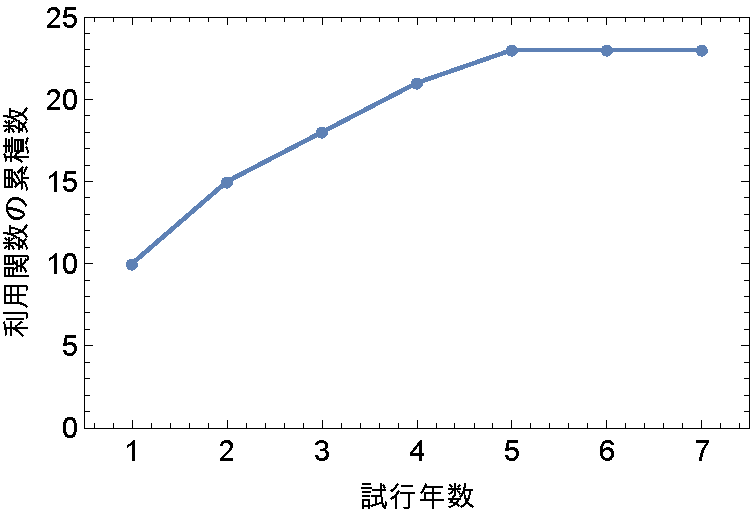
\includegraphics[scale=1.3]{code.pdf}
\caption{試行年数に対する使用関数の累積数}\label{累積グラフ}
\end{figure}

2009年から2015年までのセンター試験の数学Ⅰ・Aの問題を解き,利用したMathematicaの組み込みシンボルの累積数を記録した結果が図\ref{累積グラフ}である.

2009 年から2015 年までのセンター試験の数学Ⅰ・Aの問題を解き,利用したMathematica の組み込みシンボルの累積数を記録した結果が図2である.

\clearpage

図2より利用した組み込みシンボルは全部で23 個となった.

使用頻度順に,

\verb|Solve|(方程式を解く)

\verb|Reruce|(同値な式に置き換える)

\verb|Simplify|(簡約)

\verb|SolveAlways|(恒等式となる条件を求める)

\verb|Maxmize|(最大化)

\verb|TrigExpand|(三角関数を展開する)

\verb|TrigFactor|(三角関数をまとめる)

\verb|TrigReduce|(三角関数を書き換える)

\verb|FactorInteger|(因数を取り出す)

\verb|Divisors|(約数を求める)

\verb|Length|(リストの長さを求める)

\verb|Sqrt|(平方根)

\verb|!|(階乗)

\verb|Clear|(シンボル割り当ての解除)

\verb|Integate|(積分)

\verb|Factor|(因数分解)

\verb|Cos|(余弦)

\verb|Sin|(正弦)

\verb|SetDelayed|(関数定義)

\verb|Expand|(式の展開)

\verb|HornerForm|(ホーナー形式への変換)

\verb|Degree|(角度の変換)

であった.

\clearpage

\section{使用したシンボル}

\subsection {Solve}

Solve[expr, vars]

方程式あるいは不等式の系exprの解を変数varsについて求めようとする.

\[Solve[-a^2 -8a-13==-22,a]\]

\begin{figure}[h]
\centering
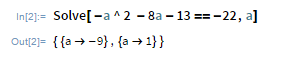
\includegraphics[width=15cm]{solve.png}
\caption{solve}\label{図}
\end{figure}

指定された変数が1つの場合,ある方程式で特定の根が1より大きい重複性を示すときは,Solveは相当する解の複数のコピーを返す.

Solve[expr,vars]は,デフォルトで,不等式に代数的に現れる数量は実数値であるが,その他の数量は複素数値であると仮定する.

Solve[expr,vars,dom]はすべての変数とパラメータが領域 dom に属すように制限する.

dom がRealsであるかIntegersやRationalsのようにその部分集合である場合,すべての定数と関数の値もまた実数に限られる.

Solve[expr,vars,Integers]は整数領域でディオファントス(Diophantine)方程式を解く.

Solve[…,x∈reg,Reals]は,領域 reg 内になるような x を含んでいる.x についての異なる座標はIndexed[x,i]で言及することができる.

expr 中の代数的変数で および互いを含まないものは,独立パラメータとして扱われる.

Solveは主として線形方程式と整方程式を扱う.

expr が実数あるいは複素数領域で整方程式と整不等式のみを含むとき,Solveは理論的には常にすべての について直接解くことができる.

expr が超越条件や整数領域を含むとき,Solveはその結果に追加的なパラメータを導入する.

Solveは整数領域上のすべての線形方程式と不等式の解の明示的な表現を与えることができ,文献に見られるディオファントス方程式の大部分を解くことができる.

expr が実数と複素数の領域上で多項式条件のみを含むとき,Solve[expr,vars]は常に限定子を除くことができる.

Solveは一般的な解のみを与える.連続的なパラメータが方程式を満足する場合にのみ有効な解は除かれる.条件付きで有効なその他の解はConditionalExpressionオブジェクトとして表される.

ConditionalExpressionの解に含まれる条件には,不等式,Element文,非連続的なパラメータについての方程式や不等式,完全次元の解を持つ方程式が含まれることがある.連続パラメータと変数についての不等式とNotElement条件は除かれる.

Solveは不等価変換を使って超越方程式の解を求める.このため,求まらない解があるかもしれず,求まった解の有効性についても厳密な条件が求められない場合もある.

Solveは,近似数値係数を持つ線形方程式の疎な系の扱いに特別の効率的な技術を用いる.




\subsection {Reduce}

Reduce[expr, vars]

varsについて方程式あるいは不等式を解き,限定子を除去することで,命題exprを簡約する.

\[Reduce[a^2 +8a+13<0,a]\]

\begin{figure}[h]
\centering
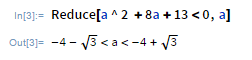
\includegraphics[width=15cm]{reduce.png}
\caption{reduce}\label{図}
\end{figure}

Reduce[expr,vars]の結果は常に と全く等しい数学的な集合を表す.

Reduce[expr,vars]はデフォルトで不等式に代数的に現れる限定子は実数で,その他の限定子は複素数であると仮定する.

Reduce[expr,vars,dom]はすべての変数とパラメータを領域 に属するものに限る.

dom がRealsであるか,あるいはIntegersやRationalsのような部分集合の場合,すべての定数と関数の値もまた実数に限られる.


Reduce[…,x∈reg,Reals]は,x が領域 reg になるように制限する.x の異なる座標にはIndexed[x,i]を使って言及することができる.

Reduce[expr,{x1,x2,…},…]は,実質的に を , , …に対する制約条件の論理結合として表現する.ただし各条件は直前ののみが関連するものとする.

中のを含まない代数的変数は独立パラメータとして扱われる.

Reduce[expr,…]の結果にLogicalExpandを適用すると,という形式の式が与えられる.ただし,各 は が定義する集合中の個々の構成要素であると考えられる.

は解体してはならないが,異なる次元を持つことはできる.LogicalExpandの後,各 は という形式になる.

LogicalExpandがなければ,Reduceはデフォルトで の条件をネストしたものを連続したレベルでOrとAndを交互に組み合せて返す.

expr が実数あるいは複素数の領域の整方程式と不等式のみを含む場合は,Reduceは原則的に常にすべての について直接解くことができる.

が超越条件や整数領域を含んでいる場合,Reduceはしばしば結果に付加的なパラメータを導入する.

が多項式条件のみを含む場合,Reduce[expr,vars,Reals]はの柱状代数分解(CAD)を与える.

Reduceは整数についてのすべての線形方程式と不等式の明示的な解の表示を与えることができ,文献中のディオファントス方程式の大部分を解くことができる.

が実数または複素数の領域で多項式条件のみを含む場合,Reduce[expr,vars]は結果に数量的変数が含まれないように常に限定子を除去する.

\clearpage

\subsection {Simplify}

Simplify[expr]

exprに対していくつかの代数的,およびその他の変数を実行し,最も簡単な形式を返す.

\[Simplify[a^2 +4a+(-13-8a-a^2 )+4]\]

\begin{figure}[h]
\centering
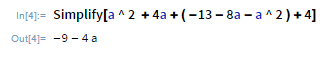
\includegraphics[width=15cm]{simplify.png}
\caption{simplify}\label{図}
\end{figure}

Simplifyは展開,因数分解やさまざまな変換を試み,その都度最も簡単な形が得られるようにする.

Simplifyは,方程式,不等式および領域指定に使われる.

不等式中の代数的な数量は,常に実数と仮定される.

FullSimplifyはSimplifyよりも強力に簡約する.

Assumingを用いてSimplifyのデフォルトの仮定を指定することができる.

仮定は,方程式,不等式,x∈Integersのような領域指定,およびこれらの論理結合からなる.

TimeConstraint->{tloc,ttot}と設定すると,最高の結果が返されるまでに,任意の特定の変換に最大t秒が,すべての変換に最大t秒が使われる.



\subsection {SolveAlways}

SolveAlways[eqns,vars]

変数 vars のすべての値について方程式 eqns を成立させるパラメータの値を与える.

\[SolveAlways[a x + b == 0, x]\]

\begin{figure}[h]
\centering
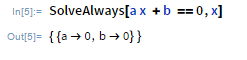
\includegraphics[width=15cm]{solvealways.png}
\caption{solvealways}\label{図}
\end{figure}

方程式は  の形式で与える.

連立方程式はリストやで組むことができる.

単一の変数,または変数のリストを指定することができる.

SolveAlwaysは,主に線形および整方程式に機能する.

SolveAlwaysは,eqns に現れるパラメータ間の関係式を作成するが,変数 vars のリストに現れるものには作成しない.

SolveAlways[eqns,vars]は,Solve[!Eliminate[!eqns,vars]]と同値である.

\subsection {Maxmize}

Maximize[f, x]

xについてfを最大にする.

\[Maximize[{-x^2 +2x+2,2<= x <= 4},x]\]

\begin{figure}[h]
\centering
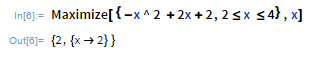
\includegraphics[width=15cm]{maxmize.png}
\caption{maxmize}\label{図}
\end{figure}

Maximizeはfの形式のリストを返す.

cons は等式,不等式,あるいはこれらの論理結合を含むことができる.

f および cons が線形あるいは多項式の場合,Maximizeは常に大域的な最大値を求める.

制約条件 cons は以下の論理結合でよい.

厳密な入力を与えると,Maximizeは厳密な結果を返す.

Maximize[{f,cons},x∈reg]は,事実上,Maximize[{f,cons∧x∈reg},x]に等しい.

 xについては,Indexed[x,i]を使って別の座標に言及することができる.
 
近似値を含む式にMaximizeが使われると,NMaximizeが自動的に呼び出される.

最大値が制約条件で定義した領域のごくわずか外側でのみ,あるいは漸近的にのみ達せられた場合,Maximizeは上限と最も近くの指定可能な点を返す.

領域が指定されていない場合,すべての変数が実数であると仮定される.

x∈Integersは特定の変数が整数値のみを取るように指定するのに使うことができる.

制約条件が満足できなければ,Maximizeは{-Infinity,{x->Indeterminate,…}}を返す.

N[Maximize[…]]は,記号的には解けない最適化問題についてはNMaximizeを呼び出す.

Maximize[f,x,WorkingPrecision->n]は n 桁精度で結果を計算する.

\clearpage

\subsection {TrigExpand}

TrigExpand[expr]

式 にある三角関数を展開する.

\[TrigExpand[Sin[2 x]]\]

\begin{figure}[h]
\centering
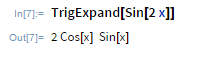
\includegraphics[width=15cm]{trigexpand.png}
\caption{trigexpand}\label{図}
\end{figure}

TrigFactorは円関数と双曲線関数のどちらにも使える.

TrigFactorは,三角関数の引数に含まれる和と整数倍の項を分離してから,可能であれば三角関数の恒等関係を使い三角関数による多項式を因数分解する.

TrigFactorは自動的に,リスト,方程式,不等式,論理関数に縫い込まれる.

\subsection {TrigFactor}

TrigFactor[expr]

式 にある三角関数を因数分解する.

\[TrigFactor[Sin[x]^2 + Tan[x]^2]\]

\begin{figure}[h]
\centering
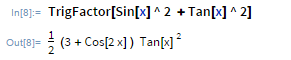
\includegraphics[width=15cm]{trigfactor.png}
\caption{trigfactor}\label{図}
\end{figure}

TrigExpandは円関数と双曲線関数のどちらにも使える.

TrigExpandは,三角関数の引数に含まれる和と整数倍の項を分離してから,可能であれば三角関数の恒等関係を使い三角関数の積をベキの和に展開する.

TrigExpandは自動的に,リスト,方程式,不等式,論理関数に縫い込まれる.

\clearpage

\subsection {TrigReduce}

TrigReduce[expr]

式 にある三角関数の積およびベキを,組み合された引数を含む三角関数に書き換える.

\[TrigReduce[2 Cos[x]^2]\]

\begin{figure}[h]
\centering
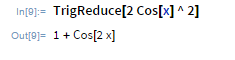
\includegraphics[width=15cm]{trigreduce.png}
\caption{trigreduce}\label{図}
\end{figure}

TrigReduceは円関数と双曲線関数のどちらにも使える.

三角関数の多項式が与えられるとき,TrigReduceは通常,引数がより複雑な三角関数の項からなる線形式を結果として与える.

TrigReduceは自動的に,リスト,方程式,不等式,論理関数に縫い込まれる.


\subsection {FactorInteger}

FactorInteger[n]

整数nの素因数をこれらの指数とともにリストとして返す.

\[FactorInteger[456]\]

\begin{figure}[h]
\centering
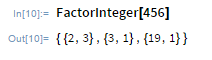
\includegraphics[width=15cm]{factorinteger.png}
\caption{factorinteger}\label{図}
\end{figure}

負の数については,単位が因数のリストに含まれる.

FactorIntegerは,有理数にも使用できる.この際,分母の素因数は負の指数とともに与えられる. 

リストFactorInteger[n,k]の最終要素は,部分因数分解後に残った部分を返す.

FactorInteger[n,GaussianIntegers->True]は,ガウスの整数上で因数分解する. 

FactorInteger[m+I n]はガウスの整数に自動的に作用する.

必要に応じて,形式,{I,1}や{-I,1}の単位が因数のリストに含まれる.

FactorInteger[n,Automatic]は見付かりやすい因数だけを取り出す.

FactorIntegerはPrimeQを使って因数が素数かどうかを確かめる.

\clearpage

\subsection {Divisors}

Divisors[n]

Nの約数となる整数をリスト形式で返す.

\[Divisors[567]\]

\begin{figure}[h]
\centering
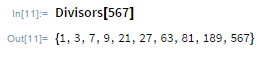
\includegraphics[width=15cm]{divisors.png}
\caption{Divisors}\label{図}
\end{figure}

Divisors[n,GaussianIntegers->True]は,約数としてガウスの整数を含む.



\subsection {Length}

Length[expr]

式exprにおける要素の数を返す.

\[Length[{1,2,3,4,5,6}]\]

\begin{figure}[h]
\centering
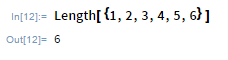
\includegraphics[width=15cm]{length.png}
\caption{Length}\label{図}
\end{figure}

expr がSparseArrayオブジェクトのとき,Length[expr]は対応する通常のリストの長さを返す.

Length[expr]は,AtomQ[expr]がTrueの場合,0を返す.

\clearpage

\subsection {Sqrt}

Sqrt[z]

または√z,zの平方根を与える.

\[Sqrt[1-(7/8 )^2 ]\]

\begin{figure}[h]
\centering
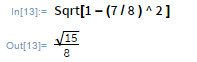
\includegraphics[width=15cm]{sqrt.png}
\caption{Sqrt}\label{図}
\end{figure}

記号操作・数値操作の両方に適した数学関数である.

√zは,Ctrl+2 zと入力できる.

Sqrt[z]は,に変換される.

$Sqrt[z^2]$は,自動的には z に変換されない.

Sqrt[a b]は,自動的にはSqrt[a]Sqrt[b]に変換されない.

これらの変換はPowerExpandを使って行うことができるが,通常,正の実数である引数に対してのみ正確である.

ある種の特別な引数については,Sqrtは自動的に厳密値に評価する.

Sqrtは任意の数値精度で評価できる.

Sqrtは自動的にリストに並列的な関数の適用を行う.

StandardFormでは$Sqrt[z]$は√zと出力される.

√z は入力に使うこともできる. √文字はEsc sqrtEscあるいは\verb|Sqrt|として入力される.


\subsection {Clear}

Clear[symbol]

Symbolに与えられている値や定義をクリアする.

\[Clear[a,b]\]

\begin{figure}[h]
\centering
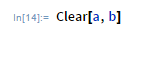
\includegraphics[width=15cm]{clear.png}
\caption{Clear}\label{図}
\end{figure}

Clearは,シンボルに結合されている属性やメッセージそしてデフォルト設定をクリアすることはない.

Clearは,次のメタキャラクタを含む省略された文字列パターンを許容する.

Clear["context`*"]は,特定のコンテキストに置かれているすべてのシンボルをクリアする.

ClearはHoldAllである.

Clearは,属性としてProtectedが与えられているシンボルに影響を与えることはない.

\clearpage

\subsection {Integrate}

Integrate[f,x]

不定積分 を与える.

\[Integrate[1/(x^3 + 1), x]\]

\begin{figure}[h]
\centering
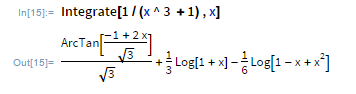
\includegraphics[width=15cm]{integrate.png}
\caption{Integrate}\label{図}
\end{figure}

$Integrate[f,x]$は$Integrate[f,x]$として入力できる.

Integrate は,Esc int Escまたは\verb|Integral|として入力できる.

dは通常のdと異なり,EscddEscまたは\verb|DifferentialD|として入力される.

$Integrate[f,{x,y,…}∈reg]$はfとして入力できる.

Integrate[f,{x,xmin,xmax}]は,xをIntegrateの下付き文字として,を上付き文字として表すことによって入力できる.

多重積分は,標準的な反復表記の変形を使用する.第1変数は,最も外側の積分に対応して与えられ,これが最後に実行される. 

Integrateは,有理関数の積分を評価することができる.また,結果が同じ関数の組で表すことができる範囲で指数関数,対数関数,三角関数,そして逆三角関数の積分を評価することができる.

Integrateは,多くの特別関数によって結果を与えることができる.

Integrateは,明示的に積分できないものについてはある種の簡約化を実行する.

定積分については,Nを適用することで数値的な結果を得ることができる. 

新しいクラスの積分に結果を与えるために,Integrateが関わるパターンに値を割り当てることができる.

積分変数はxのような構造や,頭部が数学関数ではない任意の式でもよい.

不定積分において,Integrateは,ほとんどすべてのパラメータの値に対して正しい結果を求める.


\subsection {Factor}

Factor[poly]

整数について多項式を因数分解する.

\[Factor[1 + 2 x + x^2]\]

\begin{figure}[h]
\centering
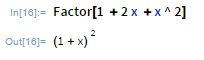
\includegraphics[width=15cm]{factor.png}
\caption{Factor}\label{図}
\end{figure}

Factorは,式の最上の代数的レベルに限って適用される.他のレベルに到達するためにはMapを使用したり,Factorを再適用したりする必要があることがある.

Factor[poly,GaussianIntegers->True]は,ガウスの整数を係数と認識し因数分解する.

poly の係数が複素数である場合,ガウスの整数を係数と認め因数分解が実行される.

変数の指数が正の整数である必要はなく,Factorは,指数が記号式の線形結合のものを取り扱うことができる.

有理式が与えられる場合,Factorは,まずTogetherを呼び出し,それから分子と分母を因数分解する.

デフォルト設定のExtension->Noneでは,Factor[poly]は多項式 poly において代数的数である係数を独立変数と同様のやり方で取り扱う.

Factor[poly,Extension->Automatic]は,多項式 poly にある任意の代数的数を含めるように,係数の取り扱える領域を拡張する. 

Factorは自動的に,リスト,方程式,不等式,論理関数に縫い込まれる.

\clearpage

\subsection {Cos}

Cos[z]

zの余弦を与える.

\[Cos[120 Degree]\]

\begin{figure}[h]
\centering
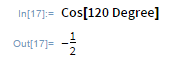
\includegraphics[width=15cm]{cos.png}
\caption{Cos}\label{図}
\end{figure}

記号操作・数値操作の両方に適した数学関数である.

明示的にQuantityオブジェクトとして与えられていない限り,Cosの引数はラジアン単位であるとみなされる(Degreeをかけて度から変換することができる). 

Cosは,引数が  の単純有理倍数である場合は自動的に評価されるが,より複雑な有理倍数の場合はFunctionExpandが使用されることもある. 

特別な引数の場合,Cosは,自動的に厳密値を計算する.

Cosは任意の数値精度で評価できる.

Cosは自動的にリストに縫い込まれる.

\subsection {Sin}

Sin[z]

Zの正弦を与える.

\[Sin[60 Degree]\]

\begin{figure}[h]
\centering
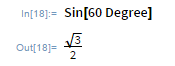
\includegraphics[width=15cm]{sin.png}
\caption{sin}\label{図}
\end{figure}

数値操作と記号操作の両方に適した数学関数である.

明示的にQuantityオブジェクトとして与えられていない限り,Sinの引数はラジアン単位であるとみなされる(Degreeをかけて度から変換することができる). 

Sinは,引数が  の単純有理数倍である場合は自動的に評価されるが,より複雑な有理数倍の場合はFunctionExpandが使用されることもある. 

特別な引数の場合,Sinは,自動的に厳密値を計算する.

Sinは,任意の数値精度で評価できる.

Sinは,自動的にリストに縫い込まれる.

\clearpage

\subsection {Tan}

Tan[z]

zの正接を与える.

\[Tan[30 Degree]\]

\begin{figure}[h]
\centering
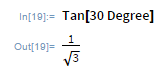
\includegraphics[width=15cm]{tan.png}
\caption{Tan}\label{図}
\end{figure}

記号操作・数値操作の両方に適した数学関数である.

Tanの引数はラジアンで与えられることを前提とする(Degreeで掛け合せることで度数から変換することができる).

Sin[z]/Cos[z]はTan[z]へ自動的に変換される.TrigFactorList[expr]は分割を行う.

Tanは引数が  の整数倍であるときは自動的に評価される.更に複雑な分数倍の場合,FunctionExpandを使う必要があることもある.

特別な引数の場合,Tanは,自動的に厳密値を計算する.

Tanは任意の数値精度で評価できる.

Tanは自動的にリストに縫い込まれる.


\subsection {SetDelayed}

SetDelayed

$rhs$を$lhs$の遅延型の値として設定する.$rhs$は,未評価の形式で維持される.$lhs$が現れると,$rhs$で置き換えられて,その都度評価される.

\[f[x_] := Expand[x^2]\]

\begin{figure}[h]
\centering
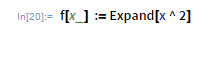
\includegraphics[width=15cm]{fx.png}
\caption{SetDelayed}\label{図}
\end{figure}

SetDelayedは属性HoldFirstではなくHoldAllを持つ.

lhsの形式の割当てをすることができる.ただし,は,それぞれの変換規則の条件や適用性を与える.同じ について複数の割当てを与えることができるが,この場合,の形式を変えて与える.

は,指定された割当てが実行可能な場合にはNullをその他の場合には$Failed$を与える.

\clearpage

\subsection {Expand}

Expand[expr]

式exprにおける積と正の整数ベキを展開する.

\[Expand[(x+1)^3]\]

\begin{figure}[h]
\centering
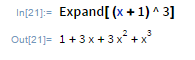
\includegraphics[width=15cm]{expand.png}
\caption{Expand}\label{図}
\end{figure}

Expandは,正の整数ベキについてのみ機能する.

Expandは,式 expr の最上レベルに限り適用される.

Expand[expr,Modulus->p]は,式 wxprを p を法として展開する. 

Expandは,方程式,不等式,論理関数と同様 expr 中のリストにも自動的に縫い込まれる.


\subsection {HornerForm}

HornerForm[poly]

多項式 poly をホーナー形式にする.

\[HornerForm[11 x^3 - 4 x^2 + 7 x + 2]\]

\begin{figure}[h]
\centering
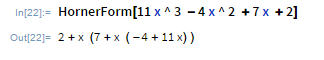
\includegraphics[width=15cm]{hornerform.png}
\caption{HornerForm}\label{図}
\end{figure}

変数が指定されていない場合,HornerFormはVariablesを用いて識別した変数について多項式あるいは有理関数をホーナー形式にする.


\subsection {Degree}

Degree

1度に対応するラジアンの数値を返す.この数値は である.

\[Cos[30 Degree]\]

\begin{figure}[h]
\centering
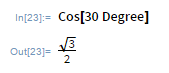
\includegraphics[width=15cm]{degree.png}
\caption{Degree}\label{図}
\end{figure}

度数をDegreeで掛け合せることによって,30 Degreeが$30 Degree$になるようにラジアンに変換することができる.

DegreeはやEsc deg Esc,\verb|Degree|等としてStandardFormおよびInputFormに入力できる.

DegreeはStandardFormではと出力される.

\clearpage

\section{利用した数学的知識}

また,利用した数学的知識は以下の表のとおりである.

\begin{table}[h]
  \begin{center}
    \caption{数学的知識}
  \begin{tabular}{|l|c|r||r|} \hline
& 2次関数 \\ \cline{2-2}
& 集合と論理・図形と計量 \\ \cline{2-2}
 2015 & データの分析 \\ \cline{2-2}
& 場合の数・確率 \\ \cline{2-2}
& 整数の性質 \\ \cline{2-2}
&図形の性質 \\ \hline
& 数と式・集合と論理 \\ \cline{2-2}
& 2次関数 \\ \cline{2-2}
 2014 & 図形と計量・平面図形 \\ \cline{2-2}
& 場合の数・確率  \\ \hline
& 数と式・集合と論理 \\ \cline{2-2}
& 2次関数 \\ \cline{2-2}
 2013 & 図形と計量・平面図形 \\ \cline{2-2}
& 場合の数・確率 \\ \hline
& 方程式と不等式・集合と論理 \\ \cline{2-2}
& 2次関数 \\ \cline{2-2}
 2012 & 図形と計量・平面図形 \\ \cline{2-2}
& 場合の数・確率 \\ \hline
& 数と式・方程式と不等式,集合と論理 \\ \cline{2-2}
& 2次関数 \\ \cline{2-2}
 2011 & 図形と計量・平面図形 \\ \cline{2-2}
& 場合の数・確率 \\ \hline
& 方程式と不等式・集合と論理 \\ \cline{2-2}
& 2次関数 \\ \cline{2-2}
 2010 & 図形と計量・平面図形 \\ \cline{2-2}
& 場合の数・確率 \\ \hline
& 数と式・集合と論理 \\ \cline{2-2}
& 2次関数 \\ \cline{2-2}
 2009 & 図形と計量・平面図形 \\ \cline{2-2}
& 場合の数・確率 \\ \hline
\end{tabular}
  \end{center}
\end{table}


\chapter{考察}

組み込みシンボルの累積数の増加が図累積グラフのように6 年で止まった.そのため,センター試験の数学I・A の問題を解くのに必要なMathematica の機能は,「結果」に記載した23 種類で十分であることがわかる.これは,センター試験の問題が一定の周期で同じ種類の問題を出題していることからもいえる.研究からも,同じような出題種類の問題は,同じ組み込みシンボルを利用していることがわかる.

\begin{figure}[h]
\centering
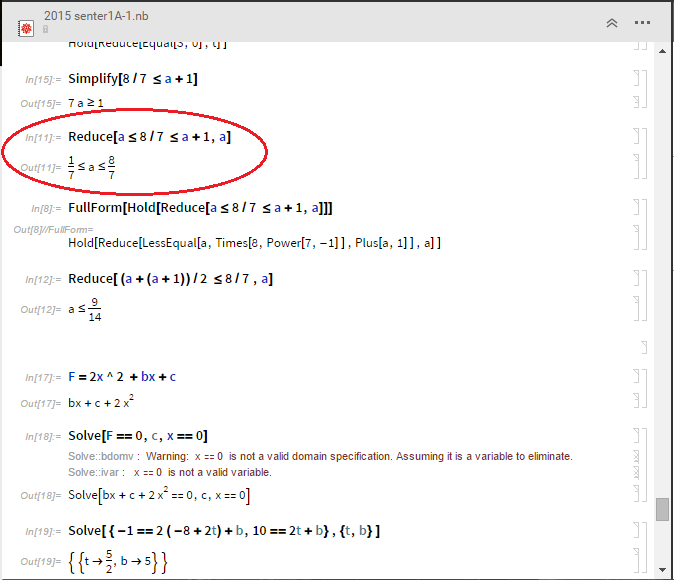
\includegraphics[width=15cm]{2013reidai.png}
\caption{2013年の問題}\label{図}
\end{figure}

\begin{figure}[h]
\centering
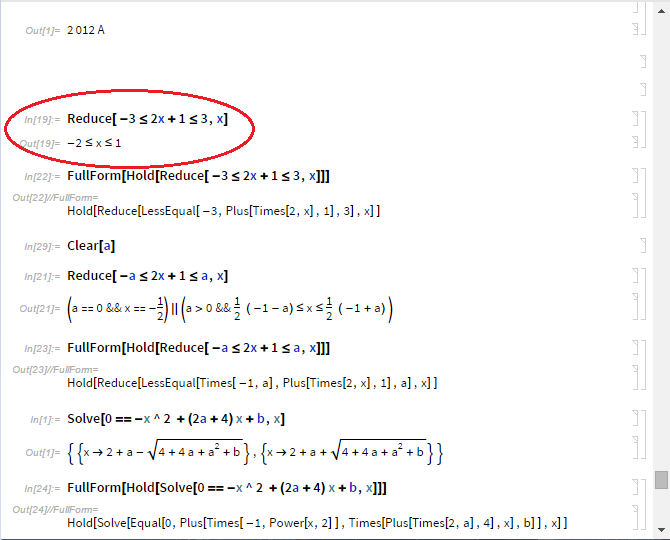
\includegraphics[width=15cm]{2012reidai.png}
\caption{2012年の問題}\label{図}
\end{figure}

この2つは違う年度であるが,同じ不等式を解く問題である.この例のように,各年度ごとに同じような問題が存在した.

\clearpage

さらに,ReduceやSolveといった組み込みシンボルは,汎用性が高く様々な種類の問題で利用された.

また,利用した数学的知識については,表で示したように,2次関数や場合の数・確率のように,各年度で毎回出題されている問題もあれば,整数の性質のように各年度で出題される種類が異なる問題もある.これにより,各年度で同じ組み込みシンボルを利用することもあるが,問題の種類に合わせた異なる組み込みシンボルを各年度で利用した.

それでも,図2のように組み込みシンボルの累積数の増加が止まるのは,2013年度と2009年度の問題の種類が同じであるように,センター試験の出題者側が周期的に問題の種類を提示しているためだと考えられる.だから,各年度で問題の種類が同じであっても組み込みシンボルの累積数の増加が止まるのであると考えられる.

Mathematicaのような数式処理システムには膨大な機能が備えられているが,数学I・A のために必要なのはこのように比較的少数の機能があり,教育の現場に導入するのも容易だと思われる.




\chapter{結論}

本研究では,数式処理システムMathematica を用いてセンター試験の数学Ⅰ・A の問題を解いた.その際に利用したMathematica の組み込みシンボルを集計することによって,センター試験の数学Ⅰ・A を解くのに必要な数式処理システムについての知識を明らかにすることができた.本研究のような事例を増やすことによって,であろう.

本研究のような事例を増やすことによって,数学教育の現場に人工知能が導入されるであろうと予測される.また,本研究では問題を理解し数学的知識で変換する作業を人間の手で行ったが,東ロボプロジェクトのように問題を人工知能が理解して回答を出すということが将来的に期待される.



参考文献は文献ファイル(この文書では\verb|biblio.bib|)に記述し,\verb|\cite|で参照する.例:データベースのための	問い合わせ言語SQLで数独を解く方法が提案されている\cite{yabuki2011}.このように参照すると,参考文献リストに自動的に登録される.文献の種類には,雑誌論文\cite{yabuki2011}や会議録論文\cite{yabuki2013},卒業論文\cite{kubo2014},書籍\cite{okumura2013},ウェブサイト\cite{self}などがある.文献の種類によって必要な項目が異なるため,\verb|biblio.bib|を見て確認すること.
参考文献は文献ファイル(この文書では\verb|biblio.bib|)に記述し,\verb|\cite|で参照する.例:データベースのための問い合わせ言語SQLで数独を解く方法が提案されている\cite{yabuki2011}.このように参照すると,参考文献リストに自動的に登録される.文献の種類には,雑誌論文\cite{yabuki2011}や会議録論文\cite{yabuki2013},卒業論文\cite{kubo2014},書籍\cite{okumura2013},ウェブサイト\cite{self}などがある.文献の種類によって必要な項目が異なるため,\verb|biblio.bib|を見て確認すること.

\bibliographystyle{junsrt}
\bibliography{biblio}%「biblio.bib」というファイルが必要.

\end{document}
